\section{Travelling Salesman Problem}
\subsection{Critic architecture}
\label{sec:appendix_tsp_critic}
The critic network architecture uses 3 attention layers similar to our encoder, after which the node embeddings are averaged and processed by an MLP with one hidden layer with 128 neurons and ReLu activation and a single output. We used the same learning rate as for the AM/PN in all experiments.

\subsection{Instance generation}
For all TSP instances, the $n$ node locations are sampled uniformly at random in the unit square. This distribution is chosen to be neither easy nor artificially hard and to be able to compare to other learned heuristics.

\subsection{Details of baselines}
\label{sec:appendix_baselines}
This section describes details of the heuristics implemented for the TSP. All of the heuristics construct a single tour in a single pass, by extending a partial solution one node at the time.

\paragraph{Nearest neighbor}
The nearest neighbor heuristic represents the partial solution as a \emph{path} with a \emph{start} and \emph{end} node. The initial path is formed by a single node, selected randomly, which becomes the start node but also the end node of the initial path. In each iteration, the next node is selected as the node nearest to the end node of the partial path. This node is added to the path and becomes the new end node. Finally, after all nodes are added this way, the end node is connected with the start node to form a tour. In our implementation, for deterministic results we always start with the first node in the input, which can be considered random as the instances are generated randomly.

\paragraph{Farthest/nearest/random insertion}
The insertion heuristics represent a partial solution as a \emph{tour}, and extends it by \emph{inserting} nodes one node at the time. In our implementation, we always insert the node using the \emph{cheapest} insertion cost. This means that when node $i$ is inserted, the place of insertion (between adjacent nodes $j$ and $k$ in the tour) is selected such that it minimizes the \emph{insertion costs} $d_{ji} + d_{ik} - d_{jk}$, where $d_{ji}$, $d_{ik}$ and $d_{jk}$ represent the distances from node $j$ to $i$, $i$ to $k$ and $j$ to $k$, respectively.

The different variants of the insertion heuristic vary in the way in which the node which is inserted is selected. Let $S$ be the set of nodes in the partial tour. \emph{Nearest} insertion inserts the node $i$ that is nearest to (any node in) the tour:
\begin{equation}
	i^* = \argmin_{i \not \in S} \min_{j \in S} d_{ij}.
\end{equation}
\emph{Farthest} insertion inserts the node $i$ such that the distance to the tour (i.e. the distance from $i$ to the nearest node $j$ in the tour) is maximized:
\begin{equation}
	i^* = \argmax_{i \not \in S} \min_{j \in S} d_{ij}.
\end{equation}
\emph{Random} insertion inserts a random node. Similar to nearest neighbor, we consider the input order random so we simply insert the nodes in this order.

\subsection{Comparison to concurrent work}
\label{app:deudon}
Independently of our work, \citet{deudon2018learning} also developed a model for TSP based on the Transformer \citep{vaswani2017attention}. There are important differences to this paper:
\begin{itemize}
    \item As `context' for the decoder, \citet{deudon2018learning} use the embeddings of the last $K = 3$ visited nodes. We use only the last (e.g. $K = 1$) node but add the \emph{first} visited node (as well as the graph embedding), since the first node is important (it is the destination) while the order of the other nodes is irrelevant as we explain in Section \ref{sec:attention_model}.
    \item \citet{deudon2018learning} use a critic as baseline (which also uses the Transformer architecture). We also experiment with using a critic (based on the Transformer architecture), but found that using a rollout baseline is much more effective (see Section \ref{sec:experiments}).
    \item \citet{deudon2018learning} report results with sampling 128 solutions, with and without 2OPT local search. We report results without 2OPT, using either a single greedy solution or sampling 1280 solutions and additionally show how this directly improves performance compared to \citet{bello2016neural}.
    \item By adding 2OPT on top of the best sampled solution, \citet{deudon2018learning} show that the model does not produce a local optimum and results can improve by using a `hybrid' approach of a learned algorithm with local search. This is a nice example of combining learned and traditional heuristics, but it is not compared against using the Pointer Network \citep{bello2016neural} with 2OPT.
    \item The model of \citet{deudon2018learning} uses a higher dimensionality internally in the decoder (for details see their paper). Training is done with 20000 steps with a batch size of 256.
    \item \citet{deudon2018learning} apply Principal Component Analysis (PCA) on the input coordinates to eliminate rotation symmetry whereas we directly input node coordinates.
    \item Additionally to TSP, we also consider two variants of VRP, the OP with different prize distributions and the (stochastic) PCTSP.
\end{itemize}

We want to emphasize that this is independent work, but for completeness we include a full emperical comparison of performance. Since the results presented in the paper by \citet{deudon2018learning} are not directly comparable, we ran their code\footnote{\url{https://github.com/MichelDeudon/encode-attend-navigate}} and report results under the same circumstances: using greedy decoding and sampling 1280 solutions on our test dataset (which has exactly the same generative procedure, e.g. uniform in the unit square). Additionally, we include results of their model with 2OPT, showing that (even without 2OPT) final performance of our model is better. We use the hyperparameters in their code, but increase the batch size to 512 and number of training steps to $100 \times 2500 = 250000$ for a fair comparison (this increased the performance of their model). As training with $n = 100$ gave out-of-memory errors, we train only on $n = 20$ and $n = 50$ and (following \citet{deudon2018learning}) report results for $n = 100$ using the model trained for $n = 50$. The training time as well as test run times are comparable.

\subsection{Extended results}
\label{sec:appendix_results_tsp}

\paragraph{Hyperparameters}
We found in general that using a larger learning rate of $10^{-3}$ works better with decay but may be unstable in some cases. A smaller learning rate $10^{-4}$ is more stable and does not require decay. This is illustrated in Figure \ref{fig:tsp_learnrates}, which shows validation results over time using both $10^{-3}$ and $10^{-4}$ with and without decay for TSP20 and TSP50 (2 seeds). As can be seen, without decay the method has not yet fully converged after 100 epochs and results may improve even further with longer training.

Table \ref{tab:results_all} shows the results in absolute terms as well as the relative \emph{optimality gap} compared to Gurobi, for all runs using seeds $1234$ and $1235$ with the two different learning rate schedules. We did not run final experiments for $n = 100$ with the larger learning rate as we found training with the smaller learning rate to be more stable. It can be seen that in most cases the end results with different learning rate schedules are similar, except for the larger models ($N=5$, $N=8$) where some of the runs diverged using the larger learning rate. Experiments with different number of layers $N$ show that $N=3$ and $N=5$ achieve best performance, and we find $N=3$ is a good trade-off between quality of the results and computational complexity (runtime) of the model.

\begin{table}
  \caption{Epoch durations and results and with different seeds and learning rate schedules for TSP.}
  \label{tab:results_all}
  \centering
  \scriptsize
  \setlength{\tabcolsep}{0.2em}
  \begin{tabular}{l|c|cccc}
    \toprule
     \multirow{2}{*}{} & epoch & \multicolumn{2}{c}{$\eta = 10^{-4}$} & \multicolumn{2}{c}{$\eta = 10^{-3} \times 0.96^{\text{epoch}}$} \\
    %\midrule
     & time & seed = 1234 & seed = 1235 & seed = 1234 & seed = 1235 \\
    \midrule
TSP20 & 5:30 & $3.85$ $(0.34 \%)$ & $3.85$ $(0.29 \%)$ & $3.85$ $(0.33 \%)$ & $3.85$ $(0.32 \%)$ \\
TSP50 & 16:20 & $5.80$ $(1.76 \%)$ & $5.79$ $(1.66 \%)$ & $5.81$ $(2.02 \%)$ & $5.81$ $(2.00 \%)$ \\
TSP100 {\small(2GPUs)} & 27:30 & $8.12$ $(4.53 \%)$ & $8.10$ $(4.34 \%)$ & - & - \\
	\midrule
N = 0 & 3:10 & $4.24$ $(10.50 \%)$ & $4.26$ $(10.95 \%)$ & $4.25$ $(10.79 \%)$ & $4.24$ $(10.55 \%)$ \\
N = 1 & 3:50 & $3.87$ $(0.97 \%)$ & $3.87$ $(1.01 \%)$ & $3.87$ $(0.90 \%)$ & $3.87$ $(0.89 \%)$ \\
N = 2 & 5:00 & $3.85$ $(0.40 \%)$ & $3.85$ $(0.44 \%)$ & $3.85$ $(0.38 \%)$ & $3.85$ $(0.39 \%)$ \\
N = 3 & 5:30 & $3.85$ $(0.34 \%)$ & $3.85$ $(0.29 \%)$ & $3.85$ $(0.33 \%)$ & $3.85$ $(0.32 \%)$ \\
N = 5 & 7:00 & $3.85$ $(0.25 \%)$ & $3.85$ $(0.28 \%)$ & $3.85$ $(0.30 \%)$ & $10.43$ $(171.82 \%)$ \\
N = 8 & 10:10 & $3.85$ $(0.28 \%)$ & $3.85$ $(0.33 \%)$ & $10.43$ $(171.82 \%)$ & $10.43$ $(171.82 \%)$ \\
	\midrule
AM / Exponential & 4:20 & $3.87$ $(0.95 \%)$ & $3.87$ $(0.93 \%)$ & $3.87$ $(0.90 \%)$ & $3.87$ $(0.87 \%)$ \\
AM / Critic & 6:10 & $3.87$ $(0.96 \%)$ & $3.87$ $(0.97 \%)$ & $3.87$ $(0.88 \%)$ & $3.87$ $(0.88 \%)$ \\
AM / Rollout & 5:30 & $3.85$ $(0.34 \%)$ & $3.85$ $(0.29 \%)$ & $3.85$ $(0.33 \%)$ & $3.85$ $(0.32 \%)$ \\
	\midrule
PN / Exponential & 5:10 & $3.95$ $(2.94 \%)$ & $3.94$ $(2.80 \%)$ & $3.92$ $(2.09 \%)$ & $3.93$ $(2.37 \%)$ \\
PN / Critic & 7:30 & $3.95$ $(3.00 \%)$ & $3.95$ $(2.93 \%)$ & $3.91$ $(2.01 \%)$ & $3.94$ $(2.84 \%)$ \\
PN / Rollout & 6:40 & $3.93$ $(2.46 \%)$ & $3.93$ $(2.36 \%)$ & $3.90$ $(1.63 \%)$ & $3.90$ $(1.78 \%)$ \\
    \bottomrule
  \end{tabular}
\end{table}

\paragraph{Generalization}
We test generalization performance on different $n$ than trained for, which we plot in Figure \ref{fig:generalization} in terms of the relative optimality gap compared to Gurobi. The train sizes are indicated with vertical marker bars. The models generalize when tested on different sizes, although quality degrades as the difference becomes bigger, which can be expected as there is \emph{no free lunch} \citep{wolpert1997no}. Since the architectures are the same, these differences mean the models learn to specialize on the problem sizes trained for. We can make a strong overall algorithm by selecting the trained model with highest validation performance for each instance size $n$ (marked in Figure \ref{fig:generalization} by the red bar). For reference, we also include the baselines, where for the methods that perform search or sampling we do not connect the dots to prevent cluttering and to make the distinction with methods that consider only a single solution clear.

\begin{figure*}[t]
\begin{center}
\centerline{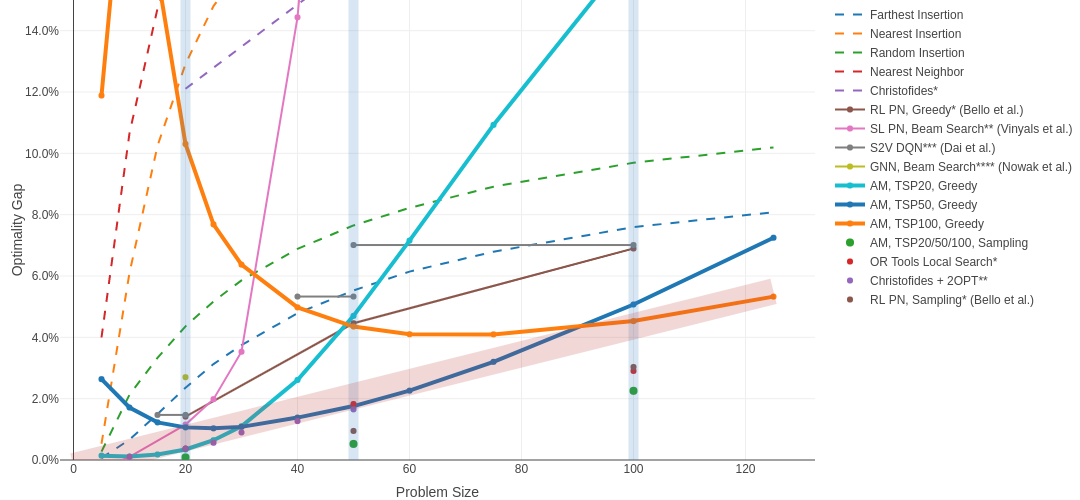
\includegraphics[trim={0 0 0 0},clip,width=\textwidth]{./images/generalization}}
\caption{Optimality gap of different methods as a function of problem size $n \in \{5, 10, 15, 20, 25, 30, 40, 50, 60, 75, 100, 125\}$. General baselines are drawn using dashed lines while learned algorithms are drawn with a solid line. Algorithms (general and learned) that perform search or sampling are plotted without connecting lines for clarity. The *, **, *** and **** indicate that values are reported from \citet{bello2016neural}, \citet{vinyals2015pointer}, \citet{dai2017learning} and \citet{nowak2017note} respectively. Best viewed in color.}
\label{fig:generalization}
\end{center}
\vskip -0.2in
\end{figure*}


\begin{figure}
    \centering
    \begin{subfigure}[b]{0.49\linewidth}
        \centerline{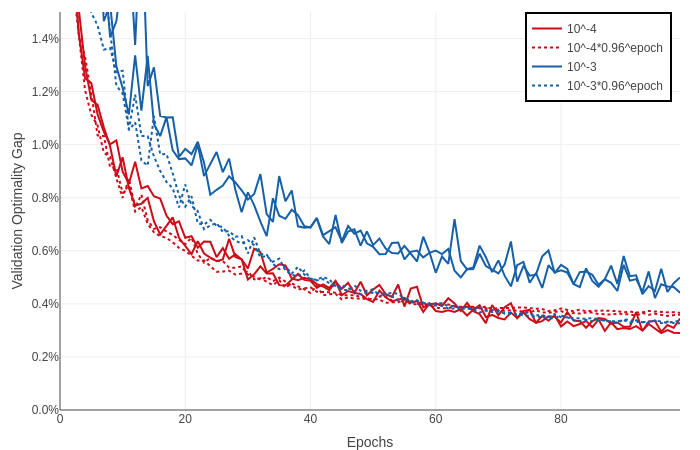
\includegraphics[trim={0 0 0 0},clip,width=\linewidth]{./images/tsp20_learnrates}}
\caption{TSP20, four schedules for $\eta$ (2 seeds)}
\label{fig:tsp20_learnrates}
    \end{subfigure}
    ~
    \begin{subfigure}[b]{0.49\linewidth}
        \centerline{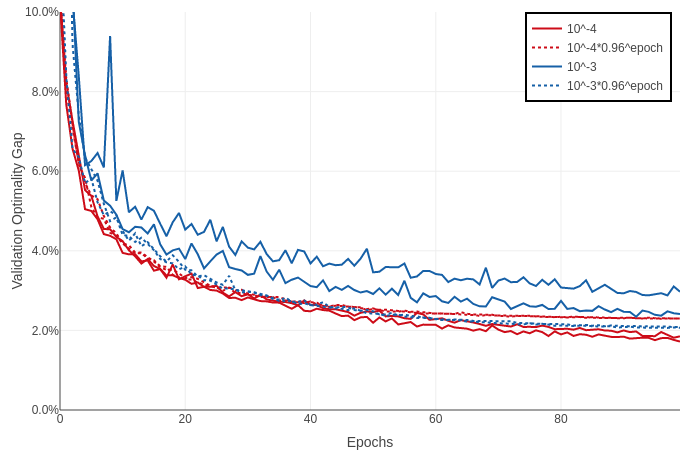
\includegraphics[trim={0 0 0 0},clip,width=\linewidth]{./images/tsp50_learnrates}}
\caption{TSP50, four schedules for $\eta$ (2 seeds)}
\label{fig:tsp50_learnrates}
    \end{subfigure}
    \caption{Validation set optimality gap as a function of the number of epochs for different $\eta$.}
    \label{fig:tsp_learnrates}
\end{figure}